
\section{Multilayer Network}

In this section, we will dive into all the unexplored paths, starting from Falkenberg's work. In particular, we will do the same polarization analysis on a topic level; instead of computing it at a full network level, we created a retweet network for each topic so we can see which are the topics that are driving the polarization of cop. Furthermore, we also want to explore how the polarization of topics evolved over time.

Thanks to the previous section now, we are familiar with the concept of topic modeling and how the main models perform. The goal is to create a multilayer network where every layer represents a topic. 

In order to do so, we developed a Python library that can be used as a toolbox starting from the tweets fresh out from the official API of Twitter. The design is modular and can achieve different goals.
In fact, even if we are interested only in the retweet network of the users (nodes are users, ties are retweets), this framework can be used to perform different tasks, but to the purpose of this study we can: 

\begin{itemize}
    \item Cluster tweets according to their topic
    \item Give a meaningful label to the clusters
    \item Create the retweet network (global and multilayer version)


\end{itemize}

The steps are independent, so, for example, you can also create the network without the need to run the topic modeling part.

\paragraph{Steps}
Even though you can skip some steps and start with your own data, the natural and minimal pipeline follows these steps:


\begin{enumerate}
    \item from JSON to a tabular format 
    \item label each tweet with a topic
    \item create multilayer retweet network  
    
\end{enumerate} 


\subsection{Process input}

The first step consists of the transformation of the JSON objects into tabular data to optimize the space and handle the data in an easier way with pandas. This is also helpful to save space; in the case of COP26, we pass from a 14GB JSON to a less than 2 GB CSV since most of the fields are not relevant to this study.

In this process, all the tweets with attachments and not in English are discarded. The tweets are divided into multiple dataframes, one for original tweets, i.e., the ones that the author actively writes, and one for the retweets.

At the end of this stage, a CSV and pkl file are saved in case somebody needs the tweets in tabular data.  If you re-run the script and these files exist, they will be loaded instead of  running again processing.

\subsection{Topic modeling}

As we extensively discussed in chapter \ref{Ch:related} in this segment of the pipeline, the tweets can be labeled using Bertopic, with the possibility to choose the embedder; the one used in this research is \textit{all-MiniLM-L6-v2}, the one evaluated in the previous section.

This step is the most computationally expensive; for this reason, to avoid redundancy, the topic modeling has been run only using original tweets. 

After this step, all the original tweets are labeled with a numeric topic, and then the label has been propagated to all the retweets so that the entire dataset is now labeled with a topic.

At this point, it is possible to use the OpenAI API to give a meaningful label to the topics; before this, it was just the most relatively frequent words of the topic. Using the langchain library, we can structure a prompt to be used.  We gave to the model the words identified with TF-IDF and 3 representative tweets sampling a subset of the documents in each topic and calculating  based on the cosine similarity between TF-IDF representations.

This is the one used: 
\\

\textit{    I want you to act as a tweet labeler, you are given representative words
from a topic and three representative tweets, give more attention to the words, all the tweets are related to climate change and COP, there is no need to mention them, detect subtopics.
start with "label:" and avoid hashtags,
which is a good short label for the topic containing the words [{words}]?, here are 3 tweets to help you:
first = "{tweet1}", second = "{tweet2}", third = "{tweet3}}
\\

Similarly to the previous stage, the labeled dataset is saved in the cache folder both in CSV and pkl. The model and the labels are saved, too.



\subsection{Network}
In this phase, after labeling the tweets, we will create a retweet network for each topic, putting all together in a multilayer network.
%The network is directed, the nodes are the users, and the tie is the number of retweets. For each topic, a network is created.

In the process of the creation of the network, there are retweeted tweets that do not have the original one, so we discard them.

The last step is the creation of a multilayer network using the multinet library developed by Uppsala University.  Every layer is a retweet network of a specific topic. It has been built starting from the subset of tweets of a specific topic, the unique users are the nodes and if user A retweets user B there will be a tie $A \rightarrow B$. The network is directed and weighted with the number of retweet. Fig \ref{fig:multilayer} is a simple example of a network with 2 layers.

The networks then has been filtered removing the outlier layer, labeled with -1.

\paragraph{COP26 network}
For cop 26 we detected 70 layers,  average number of user per layer is 8127, min is 15, max is 108829, what else?

\paragraph{COP21 Network}
like cop 26



\begin{figure}
    \centering
    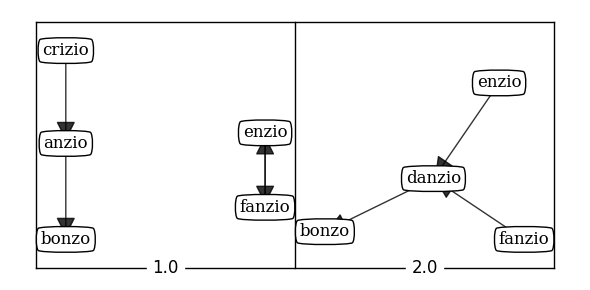
\includegraphics[width=0.75\linewidth]{Chapter4/figures/projected_topics_ml.png}
    \caption{Example of multilayer retweet network }
    \label{fig:multilayer}
\end{figure}




\section{Polarization}
At this point, for each layer, we can compute for each user a latent ideology score, and then, using Hartigan's diptest, we can assign to each topic a polarization value. More details on how this is computed are in the related works.
In this process, there are some parameters we can adjust: the number of influencers, which are defined as the most retweeted users, and $n$, which represents the minimum number of retweets a user should have done to an influencer to be considered.

The ideology score is not computed on all the users, but when selecting the influencers, we are delimiting the users to the ones that retweeted at least n times those influencers. 

In order to have enought data to analyze we set $n\_influencers = 100$ and $n=2$ . The hartigan diptest requires a minimum of nodes to be statistically significant, at this point the layer are filtered, all the layers with a p-value of the diptest higher than  0.05 have been discarded. 

\paragraph{COP26 }
COP26 we pass from 70 to 30 networks
The total influencers considered  in cop 26 in the analysis is 1698 and 22302 users have a score assigned for cop26, with an average of 1311 actors per topic, with a min of 151 and a max of 7764.  

\paragraph{COP21 to fix}
COP21we pass from 70 to 26 networks
The total influencers considered  in cop 26 in the analysis is 1557 and 22161 users have a score assigned for cop26, with an average of 1311 actors per topic, with a min of 151 and a max of 7764.  

Tab     \ref{tab:recap_ideology} presents a summary of the starting networks 


\begin{table}[h]
    \centering
    \begin{tabular}{|l|l|l|l|}
        \hline
        \textbf{Description} & \textbf{COP21} & \textbf{COP26} & \textbf{COP2x}\\ \hline
        Initial topics & 36 & 70 & 1 \\ \hline
        Final topics & 4 & 26 & 1\\ \hline
        Influencers scored & 270 & 1557 & 1\\ \hline
        Users scored & 7931 & 22161& 1 \\ \hline
        Mean users/topic &  2058 & 1311 & 1\\ \hline
        Min users/topic & 35 & 151 & 1\\ \hline
        Max users/topic & 7524 & 7764 & 1\\ \hline
        \end{tabular}
        \caption{Summary of Latent ideology}
    \label{tab:recap_ideology}
\end{table}


\section{Logitudinal analysis}
In order to see topic polarization over time, we need to run the topic modeling with all the tweets. Still, there are too many, so instead of taking the original tweets of cop 21 and cop26, we only take the original with at least one retweet which are around 1/3 of the total but are the one needed to create  the rest of the network.

Then the two dataset have been merged, we will refer to this dataset $COP2x$ and the same process described below has been done.




 
